% Full title as you would like it to appear on the page
\chapter{The Rubin Observatory Active Optics System}
\label{chap:aos}
% Short title that appears in the header of pages within the chapter
\chaptermark{Rubin Active Optics}

\epigraph{Some people don't like change, but you need to embrace change if the alternative is disaster.}{Elon Musk}

\section{Rubin Telescope}
The Vera C. Rubin Observatory is a 8.4-m wide-field telescope designed to measure the structure and evolution of the universe. The roots of the observatory date back twenty years ago to a 2001 proposal for The Dark Matter Telescope \cite{2001ASPC..237..417T}. The original scientific motivation was to produce premier weak lensing catalogs. Since then, the facility has gone through two name changes (it was the Large Synoptic Survey Telescope for many years) and the purview has expanded to include cataloging the solar system, mapping the milky way, and exploring the transient and variable sky \cite{sciencebook}. Site construction began on Cerro Pach\'{o}n, Chile in 2015 and is expected to be completed in 2023 \cite{2020SPIE11445E..0IT, 2020SPIE11445E..1US}. 

Rubin will have a $319\ \text{meter}^2\text{degrees}^2$ \'{e}tendue, ten times larger than any previous or currently planned telescope. The large \'{e}tendue is achieved by a novel three mirror design with a very fast f/1.234 beam. The design is optimized to attain seeing limited image quality across the $9.6\ \text{deg}^2$ field of view and passband spanning $320-1050\ nm$. Figure \ref{fig:telescope} shows the light path through the optics. The incident light first strikes the annular primary mirror M1, which has an outer diameter of $8.4\ m$ and an effective filled aperture of $6.4\ m$. Next the light visits the $3.4\ m$ convex secondary mirror M2 and the $5.0\ m$ concave tertiary mirror M3. Then the light passes through three refractive camera lenses and onto the $64\ cm$ focal plane. 

The primary and tertiary mirrors, M1 and M3, share an inner and outer radius respectively. This was chosen so that they could be fabricated from a single monolithic blank using spin-cast borosilicated technology. We refer to this collective mirror as M1M3. 

\begin{figure}[hbt!]
\centering
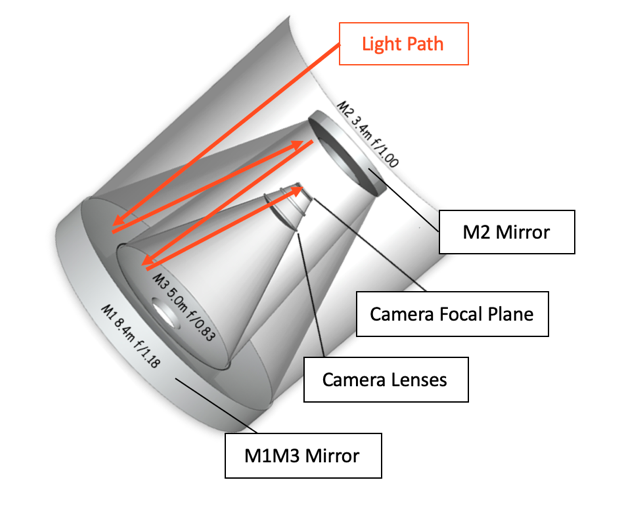
\includegraphics[width=14cm, keepaspectratio]{figs/rubin_telescope_and_aos/telescope.png}
\caption[Rubin Optics]{The optic elements of the Rubin telescope. The light path through the optics is shown in orange.}
\label{fig:telescope}
\end{figure}

\section{Active Control}

There are two telescope properties that incentivize the creation of telescopes with large primary mirrors. First, the \'{e}tendue, or light collecting power of a telescope is proportional to the area of the primary mirror. Second, the diffraction limited seeing is inversely proportional to the diameter of the primary mirror. Historically these primary mirrors were thick in order to maintain their nominal surface figure. However, the maximum size possible by these manufacturing processes is 5-6 meters of diameter.

In the late 1980s active optics technology was developed to enable the construction of a generation of telescopes with 8 meter primary mirrors. The mirrors for telescopes with this technology are thin and malleable. For Rubin, the mirrors are made out of borosilicate, which also quickly equilibrates with the ambient temperature. Active optics works by actively adjusting degrees of freedom of the telescope, including the mirror surface, based on a feedback system. The main sources of deviation to correct for are mechanical stresses stemming from the dyamics, wind, and gravity and temperature gradients in the mirror surfaces.

Figure \ref{fig:m1m3act} shows the active components of the combined primary and tertiary mirrors M1M3. The position in the x,y, and z directions is controlled by six large actuator hardpoints that form a hexapod. The mirror surface is controlled by 156 pnuematic actuators. The distribution of the actuators and their axes is explained in detail in \cite{2016SPIE.9906E..0QN}, although these details are not critical for this thesis. Given that even the large hardpoint acutators are pneumatic it is apt to say that the mirror sits on air. 

\begin{figure}[hbt!]
\centering
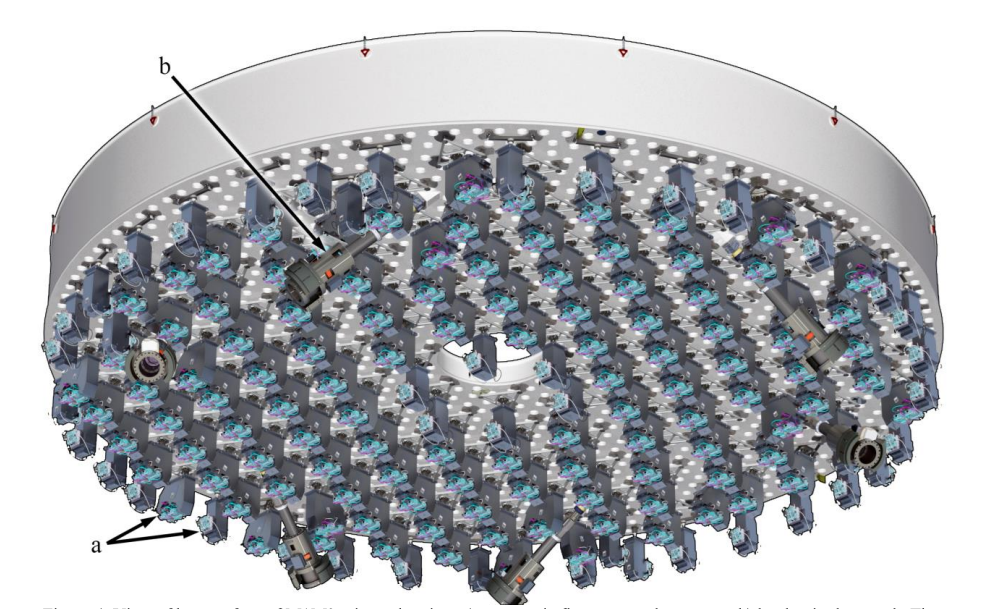
\includegraphics[width=14cm, keepaspectratio]{figs/rubin_telescope_and_aos/M1M3actuators.png}
\caption[Rubin M1M3 Hexapod and Pneumatic Actuators]{View of the bottom face of the M1M3 mirror showing: (a) pneumatic figure control actuators and (b) hard point hexapod. Source: \cite{2016SPIE.9906E..0QN}.}
\label{fig:m1m3act}
\end{figure}

Figure \ref{fig:m2act} shows the active components of the aspherical secondary mirror M2. The position in the x,y, and z directions is controlled by six large tangential electromechanical actuators. The mirror surface is controlled by 72 axial electromechanical actuators. The details of the configuration, metrology, and testing are described further in \cite{2016SPIE.9906E..67N}. Again, these details are not strictly necessary for what follows.

\begin{figure}[hbt!]
\centering
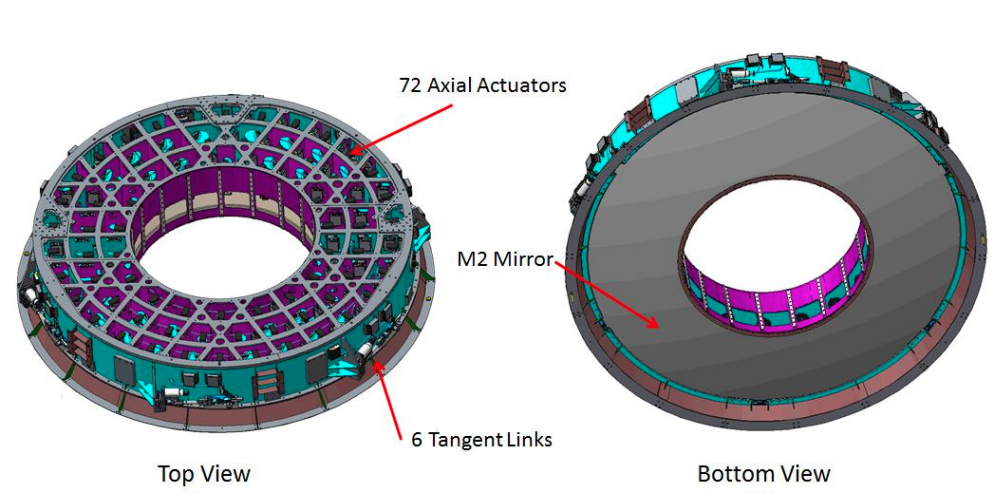
\includegraphics[width=14cm, keepaspectratio]{figs/rubin_telescope_and_aos/M2actuators.png}
\caption[Rubin M2 Hexapod and Mechanical Actuators]{Top and bottom views of the secondary mirror M2 showing the mirror cell, mirror, axial actuators, and tangential hard points. Source: \cite{2016SPIE.9906E..67N}.}
\label{fig:m2act}
\end{figure}

While it is important to understand the underlying physical interfaces for controlling the telescope, we use a key abstraction to reduce the dimensionality of the problem. Instead of modeling the state of the mirror surfaces with hundreds of predicted actuator deviations, we use low order bending modes. These are the modes that are most excited by the aforementioned sources of perturbations. Not only does this allow us to reduce the dimensionality by an order of magnitude, it also better captures the deviations we care about. We use finite element simulations to determine which modes have the most power and how many modes are required to maintain Rubin image quality specifications. 

At the time this work was initiated, all the bending modes had not been confirmed. Thus we decided to parameterize deviations to the mirror surface with the first 20 annular Zernike polynomials. We do not belive this choice has significant impact on the analysis. Table \ref{tab:dof} shows the 50 degrees of freedom - 5 for each hexapod and 20 for each mirror surface. It is worth emphasizing that this telescope's predecessor, the Dark Energy Camera on the Blanco Telescope, only controls 8 degrees of freedom. 

\begin{table}[hbt!]
\caption[The 50 Telescope Degrees of Freedom]{\label{tab:dof}The 50 telescope optics control parameters. Notation: dx is a translation in the x-axis and rx is a rotation along the x-axis.} 
\begin{center}
\begin{tabular}{|l|l|}
\hline
\rule[-1ex]{0pt}{3.5ex} Camera hardpoints & dx, dy, dz, rx, ry \\
\hline
\rule[-1ex]{0pt}{3.5ex} M2 hardpoints & dx, dy, dz, rx, ry \\
\hline
\rule[-1ex]{0pt}{3.5ex} M1M3 figure & 20 surface bending modes \\
\hline
\rule[-1ex]{0pt}{3.5ex} M2 figure & 20 surface bending modes \\
\hline
\end{tabular}
\end{center}
\end{table} 

\section{Wavefront Sensors and Donut Images}

In the last section we discussed the degrees of freedom we are trying to predict and control. In this section we describe the feedback system that makes this possible. 

The Rubin focal plane is comprised of 189 science sensors, 4 wavefront sensors, and 8 guidestar sensors \cite{10.1117/12.926710}. The wavefront sensors, in the four corners of the focal plane, are used for active optics. Each $4k\ \times\ 4k$ pixel sensor consists of two $2k\ \times 4k$ pixel half-chips. One half-chip is $1.5\ mm$ intra-focal; the other is $1.5\ mm$ extra-focal. The stars on these images are called \textit{donuts} because of their annular, donut-like shape. Figure \ref{fig:focalplane} shows the layout of the focal plane and simulated donut images.

\begin{figure}[hbt!]
\centering
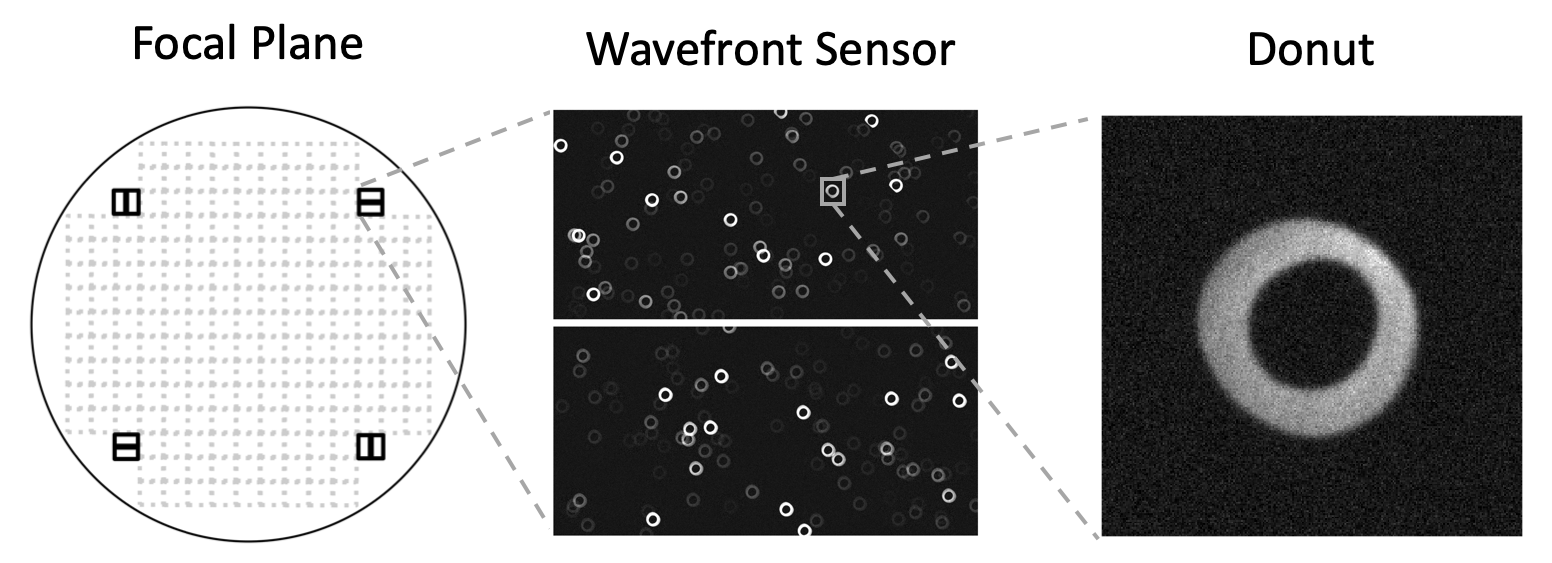
\includegraphics[width=14cm, keepaspectratio]{figs/rubin_telescope_and_aos/wavefrontsensorbreakdown.png}
\caption[From Focal Plane, To Wavefront Sensor, To Donut Image]{Left: the Rubin focal plane; science sensors are in gray; wavefront sensors are in black. Middle: One wavefront sensor split into intra-focal and extra-focal half-chips. Right: a single $256\ \times\ 256$ pixel crop of a donut.}
\label{fig:focalplane}
\end{figure}

The annular shape of the donut image stems from the outline of the M1 aperature. Figure \ref{fig:focalplane} highlights this intuition. The intra-focal and extra-focal sensors cut off the Rubin beam before it has converged. The intensity pattern in these larger images provide more information about the location of perturbations that are accounted for across the entrance pupil.

\begin{figure}[hbt!]
\centering
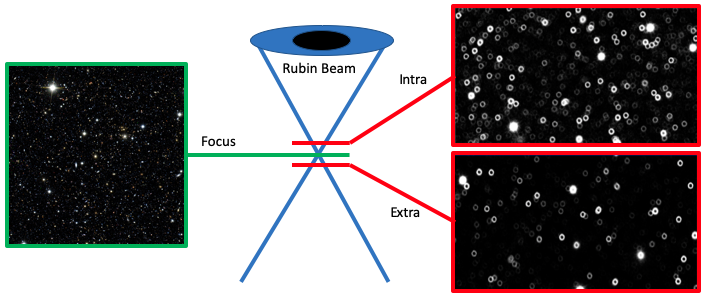
\includegraphics[width=14cm, keepaspectratio]{figs/rubin_telescope_and_aos/donutintuition.png}
\caption[Donut Image Intuition]{The images formed from placing sensors at different positions along the optical path. The optical path from the pupil to focus is shown in blue. The image produced at focus is shown in green. The intra-focal and extra-focal images are shown in red. The donut shape stems from the annular entrance pupil.}
\label{fig:focalplane}
\end{figure}


